%%%%%%%%%%%%%%%%%%%%%%%%%%%%%%%%%%%%%%%%%
% Imperial College London Poster (Portrait)
% LaTeX Template
% Version 1.0 (February 22, 2024)
%
% For current versions and to report
% issues, please see:
% https://github.com/ImperialCollegeLondon/imperial_latex_templates
%
%!TEX program = xelatex
% Note: this template must be compiled with XeLaTeX rather than PDFLaTeX
% due to the custom fonts used. The line above should ensure this happens
% automatically, but if it doesn't, your LaTeX editor should have a simple toggle
% to switch to using XeLaTeX.
%
% © Imperial College London, 2024. This template, including logo and fonts, is 
% for use of Imperial staff and students only for university business. All rights 
% reserved to the copyright owners.
%
%%%%%%%%%%%%%%%%%%%%%%%%%%%%%%%%%%%%%%%%%

%----------------------------------------------------------------------------------------
%	CLASS, PACKAGES AND OTHER DOCUMENT CONFIGURATIONS
%----------------------------------------------------------------------------------------

\documentclass[
	%print, % Uncomment to convert colors to CMYK for printing purposes
	%a1papersize, % Uncomment to use an A1 paper size instead of the default A0 paper size
]{ImperialPoster}

%----------------------------------------------------------------------------------------
%	POSTER INFORMATION
%----------------------------------------------------------------------------------------

\postertitle{Fully implicit moisture-dynamics coupling} % The poster title, can be split across multiple lines manually with \\

% Contributor/author names, can be split across multiple lines manually with \\
% Add affiliations using the \affiliation{} command
\posterauthors{Colin Cotter\affiliation{1}}

% Command to output coauthor logos to the right of the Imperial logo in the header of the poster
% If no coauthor logos are required, remove or comment out this command
\coauthorlogos{
  \coauthorlogo[4cm]{firedrake.png} % Use the optional parameter to specify a height for the logo
}

%----------------------------------------------------------------------------------------

\usepackage{biblatex}
\usepackage{amsfonts,amsopn,amsmath}
\usepackage{setspace}
\setlength{\bibitemsep}{0pt}
\addbibresource{poster.bib}
\DeclareMathOperator{\sat}{sat}
\newcommand{\pp}[2]{\frac{\partial #1}{\partial #2}}
\newcommand{\DD}[2]{\frac{D #1}{D #2}} 

\begin{document}

%----------------------------------------------------------------------------------------
%	EXAMPLE POSTER LAYOUT 1
%----------------------------------------------------------------------------------------

\titlesection % Output the title section, automatically populated using the information in the POSTER INFORMATION block above

\begin{multicols}{3} % Start the three-column layout
	
	%----------------------------------------------------------------------------------------
	%	FIRST COLUMN
	%----------------------------------------------------------------------------------------

   Instead of building complicated splitting methods between different
   dynamics and physics components, we consider applying implicit
   Runge-Kutta methods to the entire coupled system (moving the
   complexity to finding a good iterative solver). In numerical weather prediction, this
   requires reinterpretation of physics processes as terms in a
   differential equation. In particular, this has been made possible
   for some moisture parameterisations. Here we focus on the thermal
   rotating shallow water equations with moisture as an exploratory
   toy system, in particular the formulation of
   \cite{zerroukat2015moist} (see also, \cite{rostami2018improved}).
   All results are presented using Firedrake \cite{FiredrakeUserManual}
   and PETSc \cite{petsc-user-ref}.
     \vspace{-5mm}
  \section{Scalable monolithic solvers}
  \vspace{-5mm}
  A ``monolithic'' solver treats the full system of coupled variables
  without elimination. To solve the nonlinear algebraic system from an
  implicit Runge-Kutta method we use:
  \begin{itemize}[noitemsep, topsep=0pt]
  \item Nonlinear system solver: \emph{linesearch Newton},
  \item Jacobian solver (for $J$ evaluated at current Newton state):
    \emph{Preconditioned GMRES},
  \item Preconditioner: \emph{monolithic geometric multigrid (V cycle)},
  \item Multigrid smoothers: \emph{additive Schwarz method (ASM)}.
  \end{itemize}

  \subsection{ASM} The mesh is decomposed
  into overlapping patches, and the fully coupled Jacobian is solved
  independently (and hence parallelisably) on each patch. The result
  of the smoother is the sum of the solutions over all of the
  patches. In this work, a ``vertex star'' patch is used: it includes
  all of the degrees of freedom in the cells sharing one vertex,
  excluding those associated to the boundary (see Figure 1). For
  3D/vertical slice models, column patches are formed from all the
  cells sharing a vertex star patch on the horizontal base mesh (see
  \cite{cotter2023compatible}).

  \subsection{Solver performance: linearisation about current state}
  For the rotating shallow water equations on the sphere linearised
  about a state of rest, the monolithic solver converges at a rate
  that is robust to mesh refinement and changes in $\Delta t$. Figure
  1 shows the average GMRES iterations per timestep to achieve a
  residual reduction of $10^{-10}$, using the ``Williamson 5
  mountain'' initial conditions and topography, run for 1 day. A
  compatible finite element discretisation with BDM2-DG1 spaces on
  triangles is used (3 pressure DOFs and 7.5 velocity DOFs per cell), with Crank-Nicholson
  implicit timestepping.
  \vspace{-5mm}
  \begin{center}
  \parbox{6.2cm}{
    \vspace{1cm}
  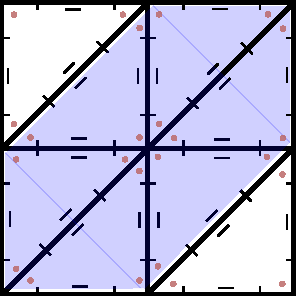
\includegraphics[width=6cm]{Images/patch}}
  \begin{tabular}{ccc}
    Cells & $\Delta t$ & its/step \\
    \hline
    20480 & 3600s & 8 \\
    81920 & 3600s & 8 \\
    327680 & 3600s & 8 \\
    20480 & 1800s & 8 \\
    20480 & 7200s & 8 \\
    20480 & 14400s & 8.6 \\
  \end{tabular} \\
  \vspace{2mm}
  {\bfseries Figure 1}: (LEFT) a diagram showing the ``vertex star'' patch. (RIGHT)
  iteration counts for the monolithic solver applied to the linear
  rotating shallow water equations on the sphere.
  \end{center}
  \vspace{-5mm}
    \subsection{Solver performance: Nonlinear rotating shallow water equations}
For the nonlinear rotating shallow water equations, the introduction
of advection terms degrades $\Delta t$ robustness but mesh independent
iteration counts are achieved upon maintaining a constant Courant
number (see Figure 2). BDM2-DG1 spaces on triangles are used
with Crank-Nicholson implicit timestepping.

  \begin{tabular}{cccc}
    Cells & $\Delta t$ & GMRES its/step & Wallclock \\
    \hline
    20480 & 3600s & 18.86 & 16m45s \\
    81920 & 1800s & 18.03 & 1h26m38s \\
    327680 & 900s & 18.00 & 9h54m50s \\
  \end{tabular} \\
  \begin{center}
      \vspace{-8mm} {\bfseries Figure 2}: Average number of GMRES
      iterations per timestep, and wallclock times, for nonlinear
      rotating shallow water equations running the ``Williamson 5
      mountain'' testcase until 15 days at various resolutions and
      fixed $\Delta x/\Delta t$ ratio, on 16 cores.
  \end{center}
  \vspace{-5mm}
\subsection{Monolithic solver for thermal rotating shallow water
  equations with moisture}

As an example, we applied the monolithic solver approach
to the model proposed in \cite{zerroukat2015moist}, which is a shallow
water model with additional active tracer variables: the potential
temperature $\theta$, water vapour $q_v$, cloud water $q_c$, and rain
water $q_r$. We discretised all the additional tracers in the same DG1
``pressure'' finite element space, and used Crank-Nicholson timestepping.
The equations take the form
\begin{align*}
  \DD{u}{t} + fk\times u + g\theta \nabla (D+b) + g\frac{D}{2}\nabla \theta
  & = 0, \\
  \pp{D}{t} + \nabla\cdot(uD) & = 0, \\
  \DD{\theta}{t} - S_\theta(q_v, q_c, \theta, D) & = 0, \\
  \DD{}{t}q_{(k)} - S_{q_{(k)}}(q_v, q_c, q_r, \theta, D) & = 0, \quad
  k=v,c,r
\end{align*}
where $S_{q_v}$, $S_{q_c}$ and $S_{q_r}$ are reaction terms governing
condensation, evaporation, and raindrop formation, and their associated
latent heat sinks/sources $S_\theta$ (see \cite{zerroukat2015moist}
for more details).

The monolithic solver for these equations is constructed exactly as for
the basic rotating shallow water equations: we use a monolithic multigrid
preconditioner with ``vertex star'' patches for ASM, now solving coupled
systems for all six variables. 

\begin{center}
  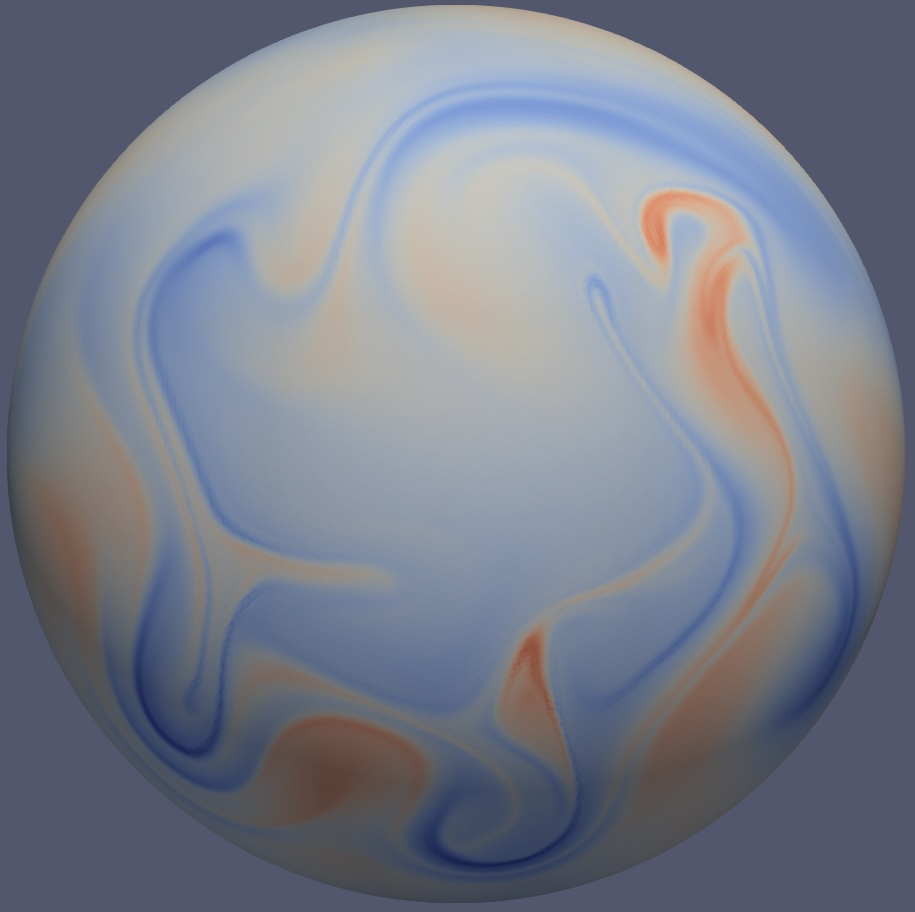
\includegraphics[height=0.45\linewidth]{vorticity6_30.jpg}
  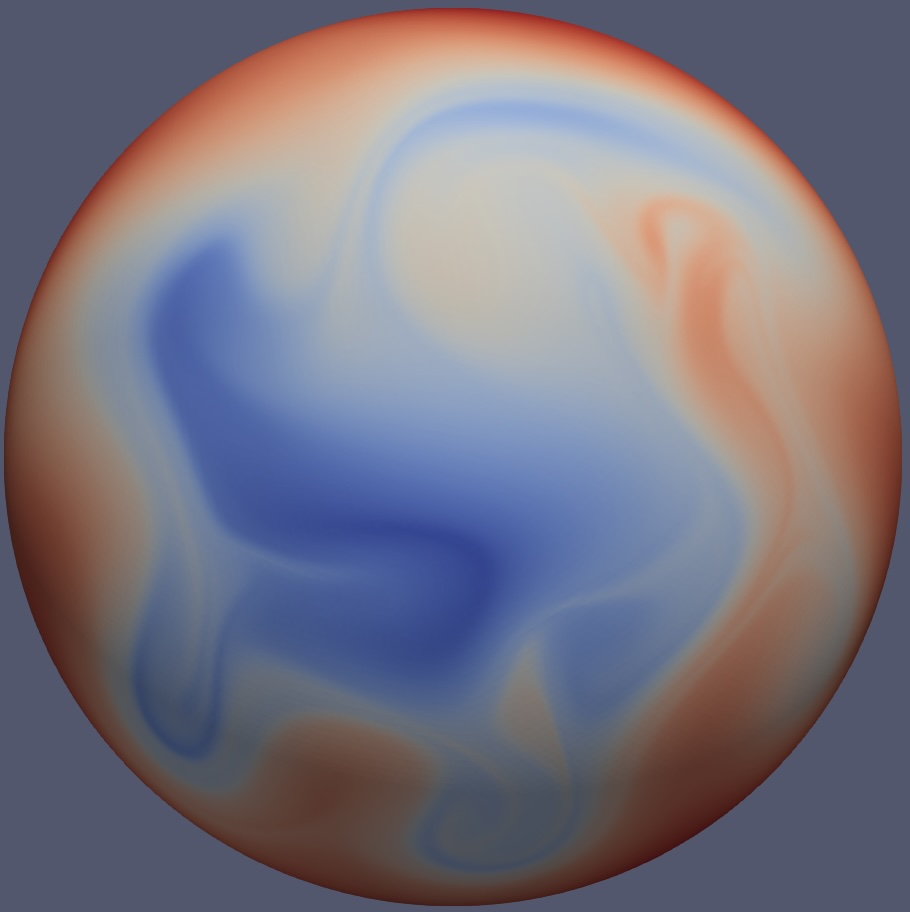
\includegraphics[height=0.45\linewidth]{elevation6_30.jpg}\\
  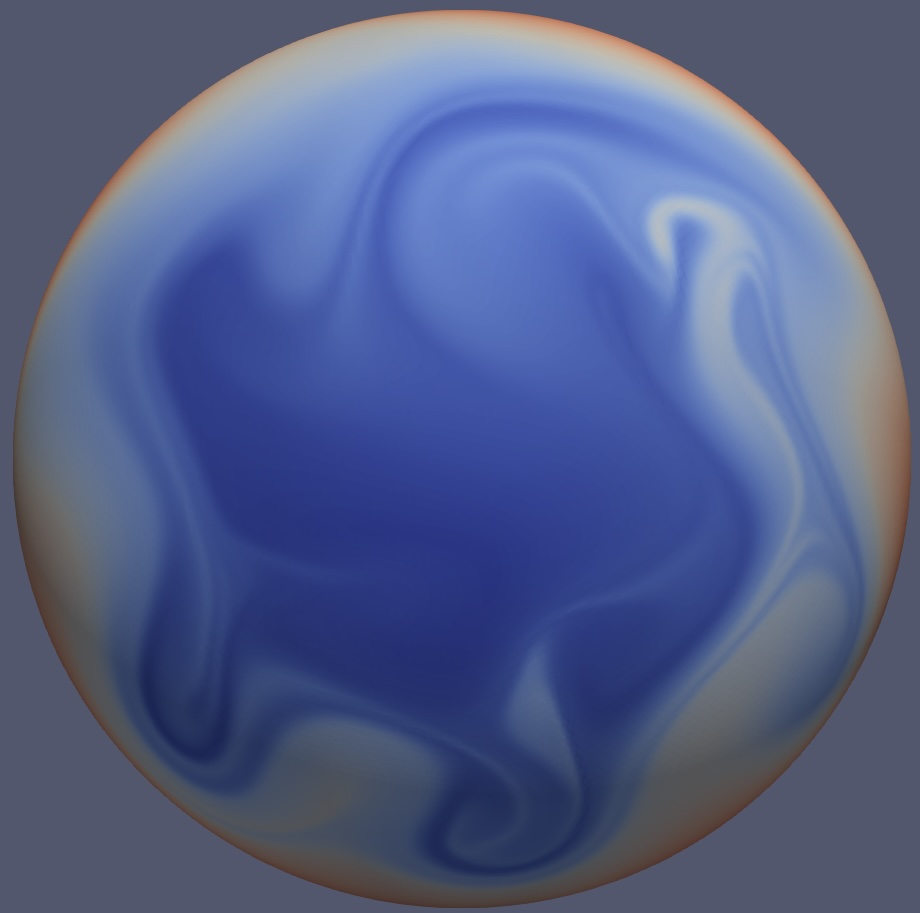
\includegraphics[height=0.45\linewidth]{vapour6_30.jpg}
  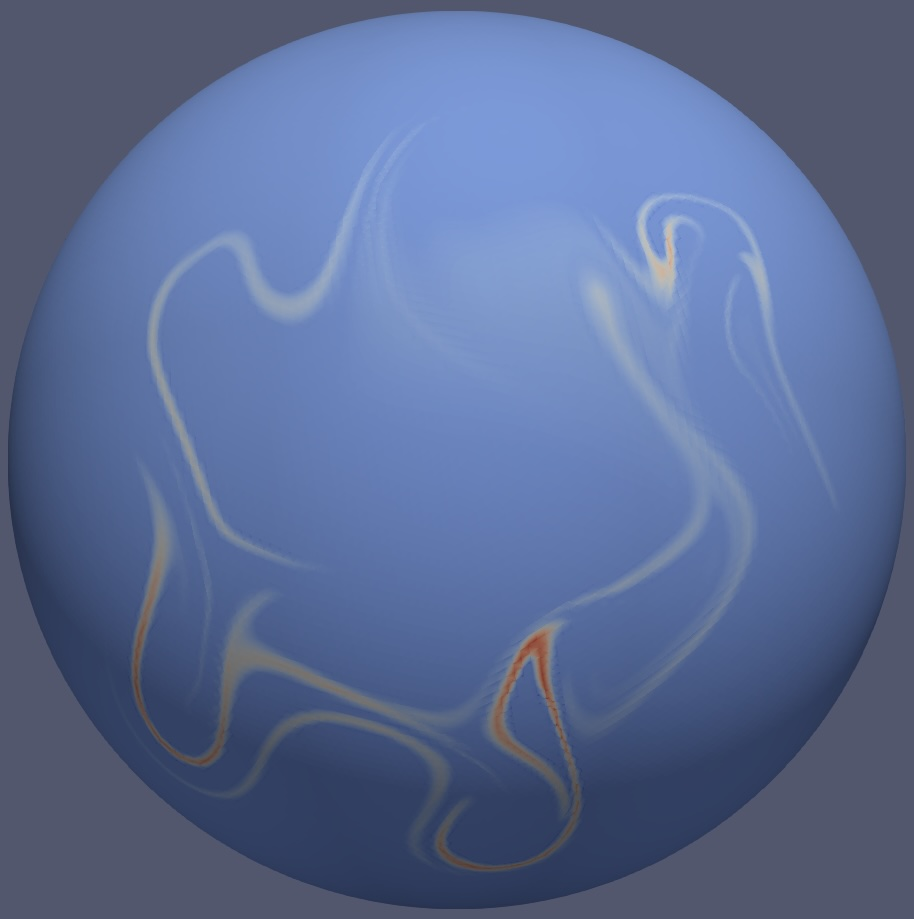
\includegraphics[height=0.45\linewidth]{cloud6_30.jpg}\\
  \begin{tabular}{cccc}
    Cells & $\Delta t$ & GMRES its/step & Wallclock \\
    \hline
    5120 & 7200s & 17.02 & 21m35s \\
    20480 & 3600s & 16.08 & 1h28m25s \\
    81920 & 1800s & 14.73 & 7h19m53s \\
  \end{tabular} \\
    \vspace{3mm} {\bfseries Figure 3}: (TOP) Solutions of the thermal
    shallow water equations with moisture, applied to the modified
    ``Williamson 5 mountain'' setup of \cite{zerroukat2015moist}, on
    81920 cells. From left to right, and top to bottom,
    the vorticity, surface elevation, water vapour and cloud are
    plotted after 30 days, all viewed from the South Pole.  (BOTTOM):
    Average number of GMRES iterations per timestep, and wallclock
    times, for these solutions until 30 days at various resolution and
    fixed $\Delta x/\Delta t$ ratio, on 16 cores.
  \end{center}

\vspace{-10mm}
\section{Differential variational inequalities for moisture}
Moisture parameterisations have saturation constraints on tracers that
are difficult to incorporate into a differential equation formulation.
This has previously been done by using Heaviside functions, or by
spreading the impulse over one timestep, as in
\cite{zerroukat2015moist,rostami2018improved}. Alternatively, we can
use the framework of differential variational inequalities
(VIs). After implicit time discretisation, these become nonlinear
complementarity problems of the form
\[
{F}({w}) \leq 0, \quad {w} \leq 0, \quad w_iF(w)_i=0, \, i=1,\ldots,N,
\]
for $F:\mathbb{R}^N\to \mathbb{R}^N$, $w\in \mathbb{R}^N$, which can
be solved using VI-adapted Newton algorithms \cite{bueler2020petsc},
which just require a suitable Jacobian solver (such as our monolithic
one).
For water vapour $q_v$ there is a maximum saturation value $q_{\sat}$
(depending on temperature etc.) so we write $q_v=q_{\sat}+q'$ with
$q'\leq 0$. This gives the VI formulation,
\begin{align*}
\DD{}{t}(q_{\sat}+q') & \leq 0,  \quad
q' \leq 0, \qquad \left[ \DD{}{t} = \pp{}{t} + u\cdot \nabla\right] \\
\DD{}{t}(q_{\sat}+q')q' & = 0, 
\end{align*}
i.e. at each point space and time, either the constraint is satisfied,
or the transport equation holds.
The rate of condensation of vapour $q_v$ into cloud $q_c$ is $R$, where
\[
\DD{}{t}(q_{\sat}+q') = -R, \quad
\DD{}{t}q_c = R \implies
\DD{}{t}q_c = -\DD{}{t}(q_{\sat}+q').
\]
\emph{\bfseries The rate $R$ is eliminated and we never need to calculate it.}
We can also use this to set the latent heat release,
\[
\DD{}{t}\theta = LR = -L\DD{}{t}(q_{\sat}+q'),
\]
where $\theta$ is potential temperature, and $L$ is a heat release constant.


Cloud evaporates back into vapour at rate $\gamma q_c$, provided that
$q'<0$. Incorporating this gives
\begin{align*}
  \DD{}{t}(q_{\sat}+q') - \gamma q_c & \leq 0, \quad
  q' \leq 0, \\
  \DD{}{t}q_c + \underbrace{\DD{}{t}(q_{\sat}+q') - \gamma q_c}_{\mbox{condensation}} + \underbrace{\gamma q_c}_{\mbox{evaporation}} & = 0, \\
  \DD{\theta}{t} + L\left(
  \underbrace{\DD{}{t}(q_{\sat}+q') - \gamma q_c}_{\mbox{condensation}} + \underbrace{\gamma q_c}_{\mbox{evaporation}}\right) & = 0, 
\end{align*}
Finally we assume a (fixed) maximum cloud value $q_p$, above which
cloud is converted to rain, $q_r$. This is achieved using another VI
for $q_c$, leading to the following
coupled system (following the framework of \cite{zerroukat2015moist} as an example),
\begin{align*}
  \DD{u}{t} + fk\times u + g\theta \nabla (D+b) + g\frac{D}{2}\nabla \theta
  & = 0, \\
  \pp{D}{t} + \nabla\cdot(uD) & = 0, \\
  \DD{\theta}{t} + L\DD{}{t}(q_{\sat}(D,\theta)+q') & = 0, \\
  \DD{}{t}(q_{\sat}(D,\theta)+q') - \gamma q_c & \leq 0, \quad q'\leq 0 \\
  \DD{}{t}q_c + \DD{}{t}(q_{\sat}(D,\theta)+q') & \leq 0, \quad
  q_c \leq q_p, \\
  \DD{q_r}{t} + \left(\DD{}{t}q_c + \DD{}{t}(q_{\sat}(D,\theta)+q')\right) & = 0,
\end{align*}
where $u$ is the (horizontal) velocity, $f$ is the Coriolis parameter,
$k$ is the local up direction, $D$ is the layer depth, $b$ is the
bottom topography, and $g$ is gravitational acceleration. This is a
{\bfseries completely time continuous system}, which can be discretised by
implicit Runge-Kutta methods, treating
the VI constraints from the DAE perspective \cite{kirby2024extending}.

\section{Summary and outlook}

We demonstrated a scalable monolithic solver approach for implicit
time integration of coupled dynamics and moisture physics in an
example rotating shallow water model.  We also presented a
differential variational inequality formulation of moisture
physics. After implicit time discretisation, the system can be solved
using an VI-adapted Newton method; this is possible using the scalable
monolithic solver. We will investigate this approach in future work,
and develop it towards other formulations, and vertical slice and 3D
models with moisture. We will also investigate other timestepping methods
such as TR-BDF2.

\vspace{-10mm}
\paragraph{Acknowledgements} CJC is grateful to Nell Hartney and Jemma Shipton for their assistance in setting up the moisture test case.

\AtNextBibliography{\small} \printbibliography
        
\subsection{Affiliations}

% Affiliation institutions, the first parameter is the affiliation number (matching the author list) and the second is the institution
\affiliationentry{1}{Department of Mathematics, Imperial College London}
	
\subsection{Funders}


\includegraphics[width=0.55\linewidth]{UKRI_logo.png} % Side by side funder logos

\includegraphics[width=0.3\linewidth]{excalibur.png} % Side by side funder logos
	
%----------------------------------------------------------------------------------------

\end{multicols}

%----------------------------------------------------------------------------------------

\end{document}
